\documentclass[amsmath,amssymb,notitlepage,12pt]{revtex4}
\usepackage[toc,page]{appendix}
\usepackage{graphicx}
\usepackage{bm}% bold math
\usepackage{multirow}
\usepackage{booktabs}
\usepackage{verbatim}
\usepackage{xcolor}
\usepackage{hyperref}
\usepackage{setspace}
\usepackage{enumitem}
\usepackage{changepage}
\hypersetup{pdftex,colorlinks=true,allcolors=blue}
\usepackage{hypcap}
\usepackage[small,compact]{titlesec}
\setlist[enumerate]{itemsep=0mm}
\newcommand{\ibeam}{20 nA\ }
\newcommand{\easy}{1.5\%}
\begin{document}
\title{Hall B M{\o}ller Operations Manual - v1.14}
\date{\today}
\author{N. Baltzell, S. Stepanyan}
\begin{abstract}
\end{abstract}
\maketitle

\tableofcontents

\newpage 

\section{General}

The Hall B M{\o}ller system measures CEBAF beam polarization in the upstream tunnel of Hall B, and this document details its operating procedures.  The user interface is shown in Fig.~\ref{fig:unconfig} and provides direct access to all necessary controls and feedback for the M{\o}ller system, and its operating procedures are detailed in Section~\ref{sec:proc}.

\begin{figure}[htbp]\centering
    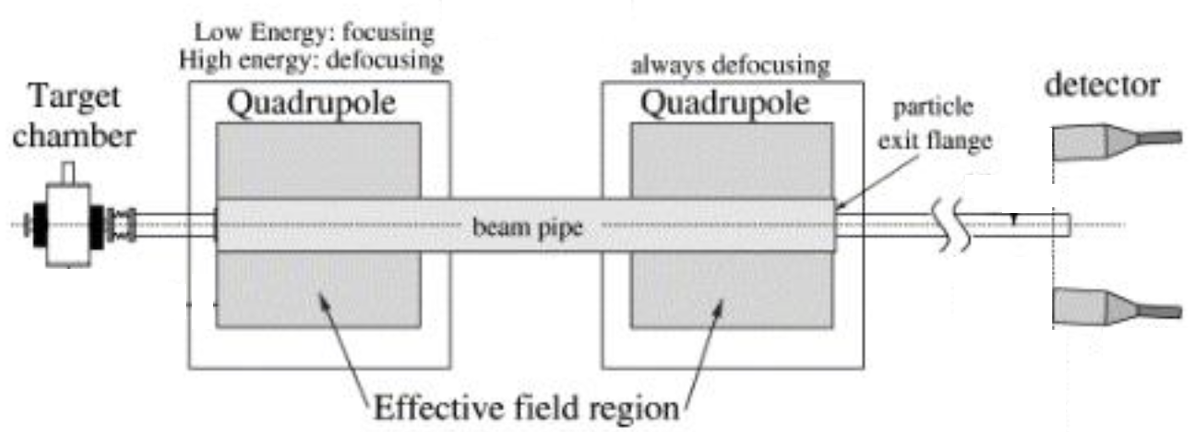
\includegraphics[width=9cm]{pics/layout}
    \caption{\label{fig:layout}Layout of the Hall B M{\o}ller system.}
\end{figure}

\section{Prerequisites}\label{sec:prereq}

\subsection{General}

M{\o}ller runs first require continuous-wave (CW) beam already delivered to the Hall B tagger dump/yoke.  Standard Hall B beamline documentation and requirements should be followed to establish that beam;  see the run wiki.

\begin{table}[htbp]\centering
    \begin{tabular}{c|c}\toprule[1.5pt]
        Beam Destination & Tagger Dump / Yoke \\
        Harps Scans & Ok: 2C21 and 2C24\\ 
        \bottomrule[1.5pt]
    \end{tabular}
    \caption{General beamline prerequisites for M{\o}ller runs.}
\end{table}

\subsection{Specific}

After establishing beam, M{\o}ller measurements require the Hall B orbit locks be disabled and the Fast ShutDown (FSD) for our Halo counters and Beam Offset Monitor (BOM) masked.  {\bf\em Note, orbit locks and FSD must be manually restored to standard settings after a M{\o}ller run.}

\begin{table}[htbp]\centering
    \begin{tabular}{c|c}\toprule[1.5pt]
        Orbit Locks & OFF\\
        FSD & Halo \& BOM Masked\\
        Beam Current & \ibeam \\
        \bottomrule[1.5pt]
    \end{tabular}
    \caption{M{\o}ller-specific beamline prerequisistes.}
\end{table}

\newpage

\section{Procedure}

\subsection{Overview}

{\em Note, if the system presents error status messages, pause beam delivery and do not resume without guidance from the Hall B beamline or slow controls experts!!}
\begin{enumerate}
    \vspace{-4mm}\item {\bf Prerequisites:}  Ensure the prerequisites of Section~\ref{sec:prereq} are satisfied
    \vspace{-4mm}\item {\bf Request No Beam:}  Ask MCC to take beam away for a configuration change
    \vspace{-4mm}\item {\bf Configure:}  Ensure the Configuration section is set as desired
    \vspace{-4mm}\item {\bf Enter:} Click \textcolor{blue}{\em Enter} and wait for success status
    \vspace{-4mm}\item {\bf Request Beam:} Ask MCC to resume beam delivery at \ibeam for M{\o}ller runs
    \vspace{-4mm}\item {\bf Start Run:} With stable beam, click \textcolor{blue}{\em Start Run}
    \vspace{-4mm}\item {\bf Monitor:} Monitor the quality requirements and reach \easy\ polarization error
    \vspace{-4mm}\item {\bf End Run:} Click \textcolor{blue}{\em End Run}
    \vspace{-4mm}\item {\bf Logbook Entry:} Input user name(s) and click \textcolor{blue}{\em Submit}
    \vspace{-4mm}\item {\bf Request No Beam:} ask MCC to take beam away for a configuration change
    \vspace{-4mm}\item {\bf Reconfigure:} (Optional) Go to step 3
    \vspace{-4mm}\item {\bf Exit:} Click \textcolor{blue}{\em Exit} and wait for success status
\end{enumerate}

\begin{figure}[htbp]\centering
    \includegraphics[width=13cm]{pics/unconfig}
    \caption{\label{fig:beamline}The user interface in the normal, non-M{\o}ller, beamline configuration.  It is divided into {\em Status}, {\em Configuration}, {\em Data Acquisition}, {\em Monitoring}, and {\em Logbook} sections.\label{fig:unconfig}}
\end{figure}

\subsection{Full}\label{sec:proc}

\begin{enumerate}\singlespacing
    \item {\bf Prerequisites:}  Ensure the prerequisites in Section~\ref{sec:prereq} are satisfied.
    \item {\bf Request No Beam:}  Ask MCC to take beam away for a configuration change \label{step:config}.
    \item {\bf Configure:}  Ensure the Configuration section is set as desired.
        See Table~\ref{tab:pars} for standard values, and check the short-term plan on the run wiki.  Contact the Run Coordinator if uncertain.
    \item {\bf Enter:} Click \textcolor{blue}{\em Enter} and wait for success status.
        This will initiate a sequence including turning off CLAS12 high voltage, inserting the blank collimator, energizing the M{\o}ller quadrupoles and Helmholtz magnets, and inserting the M{\o}ller target.
        \begin{adjustwidth}{1cm}{1cm}
            {\em Success will result in \textcolor{green}{\em Moller Configuration Ready} in the status message, otherwise first ask MCC to pause beam, and then contact the Hall B slow controls or beamline expert for guidance before proceeding!}
        \end{adjustwidth}
    \item {\bf Request Beam:} Ask MCC to resume beam delivery at \ibeam for M{\o}ller runs.
    \item {\bf Start Run:} With stable beam, click \textcolor{blue}{\em Start Run}\label{step:start}.
        This will initiate a sequence including zeroing any accumulated data, opening a new data file, incrementing the run number, and starting data acquisition.
    \item {\bf Monitor:} Monitor the quality requirements and reach \easy\ polarization error
        Refer to Table~\ref{tab:reqs} for the requirements, e.g., beam charge asymmetry and accidental ratio, and possible remedies in Section~\ref{sec:knobs}.
        Contact the beamline expert for guidance if necessary.  
    \item {\bf End Run:} Click \textcolor{blue}{\em End Run}.  At this point you should be in one of 3 states:
        \begin{enumerate}
            \item Achieved the desired polarization error of \easy\ $\to$ Go to \#\ref{step:log} (Logbook Entry)
            \item Need to start a new M{\o}ller run, no configuring $\to$ Go to Step \#\ref{step:start} (Start Run)
            \item Need to reconfigure the M{\o}ller system $\to$ Go to Step \#\ref{step:reconfig} (No Beam)
        \end{enumerate}
    \item {\bf Logbook Entry:} Input your name(s) and click \textcolor{blue}{\em Submit}\label{step:log}.
        This will submit a tagged, searchable log entry to HBLOG with a table summarizing the results and an attached data file, and requires filling the {\em Entry Makers} field!
    \item {\bf Request No Beam:} ask MCC to take beam away for a configuration change \label{step:reconfig}.
    \item {\bf Reconfigure:} (Optional!) $\to$ Go to step 3
    \item {\bf Exit:} Click \textcolor{blue}{\em Exit} and wait for the success status.  
        This will restore the non-M{\o}ller beamline configuration by turning off the quadrupoles and Helmholtz magnets and retracting the M{\o}ller target.  
        \begin{adjustwidth}{1cm}{1cm}
            {\em Success will result in \textcolor{green}{\em Non-M{\o}ller Configuration} in the status message, otherwise contact the Hall B slow controls or beamline expert for guidance before proceeding!}
        \end{adjustwidth}
        Note, CLAS12 detector high voltage, Hall B orbit locks, and FSD configuration will need to be restored manually.
\end{enumerate}

\section{Quality Requirements}\label{sec:quality}

The requirements to be maintained during a M{\o}ller run, and the resulting desired error on the polarization measurement are shown in Table~\ref{tab:reqs}.  It is the responsibility of the operator to monitor these quantities to ensure a successful polarization measurement.

\begin{table}[htbp]\centering
    \begin{tabular}{ll}\toprule[1.5pt]
        2C21 BPM Current & $\sim$\ibeam\\
        Beam Charge Asymmetry & $<0.2\%$ (typical $\sim 0.1\%$)\\
        Accidental/Coincidence Ratio & $<0.1$ (typical $\sim 0.05$)\\
        Final Beam Polarization Error & $<$\easy (absolute)\\
        \bottomrule[1.5pt]
    \end{tabular}
    \caption{Standard quality conditions required for a M{\o}ller run.  Live values are shown in the {\em Monitoring} and {\em Data Acquisition} sections in Figure~\ref{fig:unconfig}.  Note, beam polarization error depends on statistics and should gradually decrease during the run.\label{tab:reqs}}
\end{table}

\subsection{Adjustable Parmaeters}\label{sec:knobs}

If quality requirements are not satisfied (accidental rate and beam charge asymmetry), first check whether our hardware settings are as expected by comparing to the parameters earlier in this document and also to recent satisfactory M{\o}ller runs in the logbook.  The following subsections contain information on the quality measurements and the main parameters that can affect them.  Consult with the Run Coordinator or beamline expert for advice on tuning these parameters, and compare their values with previous M{\o}ller runs.

\subsection{Run Duration}

With 20 nA, 11 GeV electron beam, the normal run duration to achieve \easy\ absolute error on the polarization is about 15 minutes of continuous beam.  Interruptions to beam delivery, e.g. trips, will of course increase the necessary run time.  Much longer than normal run duration can be indicative of excessive accidentals or beam charge asymmetry.

\subsection{Beam Charge Asymmetry}

Beam charge asymmetry is measured by a Synchrotron Light Monitor fed to a Struck scaler latching on the heliticy signals.  The SLM is located a few meters upstream of, and {\em completely independent of}, the rest or our M{\o}ller system.  Beam Charge asymmetry is affected primarily by beam characteristics from the injector and accelerator.  There can be some effect from quality of the SLM performance, e.g. if voltage is far too high and the SLM is saturated, but this should generally never be the case for the normal operator.

Note that beam charge asymmetry updates with the same period as our Moller acquisition time, i.e. if the acquisition time is set at 60 seconds, beam charge asymmetry will only update once per minute.

If the beam charge asymmetry is too high, the parameters that can be considered are:

\begin{itemize}
    \vspace{-4mm}\item Beam position (BPM and harp scans)
    \vspace{-4mm}\item Beam profile (harp scans)
    \vspace{-4mm}\item Injector slit setting
    \vspace{-4mm}\item Injector attenuator settings
\end{itemize}

\subsection{Accidentals}

The accidental-coincidence ratio is measured by M{\o}ller Left/Right PMTs, downstream of the target and quadrupoles, and is independent of the helicity signals.  Excessive accidentals can be caused by beam quality issues, e.g. bleedthrough from other halls, or non-optimal settings of our M{\o}ller system.  Parameters that can be considered for adjustment include the same beam quality parameters in the previous section, and with the addition of our M{\o}ller configuration, e.g. Left/Right PMT voltages, malfunctioning quadrupoles, or very miscalibrated target position.

\section{Hardware Settings}

The standard hardware settings for a M{\o}ller run are shown in Table~\ref{tab:pars}.  These are displayed in the {\em Configuration} section of Figure~\ref{fig:unconfig} and will be used to automatically configure all hardware during the procedure in Section \ref{sec:proc}.  In case of any inconsistency with parameters in this table, check with the beamline or slow controls expert.

\begin{table}[htbp]\centering
    \begin{tabular}{ll}\toprule[1.5pt]
        SLM Voltage & 1400 V \\
        Target Position & Left or Right \\
        Helmholtz Current & $\pm$3.5 A \\
        Quadrupole Current & Auto \\
        \bottomrule[1.5pt]
    \end{tabular}
    \caption{Standard parameter values for configuring the M{\o}ller setup. {\em  Note, the ``Auto'' setting for the quadrupoles uses the beam energy dependence in Figure~\ref{fig:quadenergy}}.\label{tab:pars}}
\end{table}

\begin{figure}[htbp]\centering
    \includegraphics[width=14cm]{pics/moller_quad_current}
    \caption{\label{fig:quadenergy}The calculated optimal quadrupole current as a function of beam energy.  This function is used if the {\em Auto} checkbox is selected in the {\em Configuration} section of Figure \ref{fig:unconfig} when entering or reconfiguring the M{\o}ller setup.  The equation can be found at \url{https://github.com/JeffersonLab/clas12-epics/blob/main/apps/mollerSetupApp/src/quadCurrent.c}.}
\end{figure}

\end{document}

